%! TeX root = master.tex
% !TEX program = lualatex

\lecture{1}{2026-02-17}{Introduction}{}
\chapter{Introduction}%
\label{cha:hop la}

\section{What is Machine Learning ?}
Machine learning = Data \textrightarrow Algorithms \textrightarrow Insight
\subsection{Data}%
\label{sub:Data}

Data = attributes/tabular, text, speech, images, mixed.

\begin{definition}[Data sample]
  An individual observation. E.g., an image, or a list of attributes for one patient
\end{definition}
\begin{definition}[Data set]
  A collection of multiple data sample. E.g., a collection of images, the attribute lists for multiple patients.
\end{definition}

\textbf{Unsupervised data} : Each sample consists only of an observation, e.g., an image (without information about its content). \\
\textbf{Supervised data} : Each sample comes with additional annotations, e.g., category label.

\subsection{Insight (what we discover from the datas)}%
\label{sub:Insight}
What insight ?
\begin{itemize}
  \item Precise, concrete prediction. E.g., the category depicted by an image.
  \item Better understanding of a phenomenon. E.g., identify the mother's charasteristics that lead to low birth weight.
  \item Better understanding of data. E.g., analyze the influences between different musical genres.
  \item \textbf{in this course} we mostly focus on precise insights. In particular we will study two classes of ML problems : \textbf{regression} and \textbf{classification}
\end{itemize}

\textbf{Regression} : Predict continuous value(s) for a given sample. E.g., predict the birth weight of a baby, human pose estimation : predict the 3D positions of human joints (multiple values). \\ 
\textbf{Classification} : Predict one discrete label for a given sample. E.g., binary classifications for movies (like vs not like; 1 or 0), muti-class image recognition (cat vs tree vs car; 0 vs 1 vs 2).

\textbf{Order}: \\ 
In regression, the values typically follow an order. E.g, predicting a weight of 3002g insted of 2977g is better that predicting 2500g. \\ 
In classification, the categories do not follow an order. E.g, predicting a ``tree'' instead of a ``cat'' is just as wrong as predicting ``car''. \textrightarrow here it's true or false.

\subsection{Algorithms}%
\label{sub:Algorithms}
What (classes of) algorithms ?
\begin{itemize}
  \item Supervised learning : \begin{itemize}
    \item Relies on supervised data
    \item The annotations typically correspond to the desired insight
  \end{itemize}
\item Unsupervised learning : \begin{itemize}
  \item Relies on unsupervised data
  \item The goal is rather to analyze the observed data set 
\end{itemize}
\end{itemize}

\textbf{Unsupervised learning}:
\begin{itemize}
  \item Single stage: Analyze the whole data or transform it for further analysis.
\end{itemize}

\textbf{Supervised learning}:
\begin{itemize}
  \item Stage 1: Training: Use data with ground-truth (info that is true) labels to optimize model parameters.
  \item Stage 2: Testing: Predict the output for a new data sample.
  \item Assumption : The annotations (correct responses) are the insight that we seek to obtain from the data. E.g.,: category label, human pose
\end{itemize}

\textbf{Training set vs test set}:
\begin{itemize}
  \item The training set and the test set should always be \textbf{completely separate}.
  \item Never use the test annotations during training \textrightarrow the test set is not to train or to improve the performance of the model, but only to test his efficiency.
  \item Assumption: they are both drawn from the same statistical distribution. E.g., digit recognition: A model trained on MNIST will work poorly on Street
View House Numbers
\end{itemize}
\begin{figure}[htpb]
  \centering
  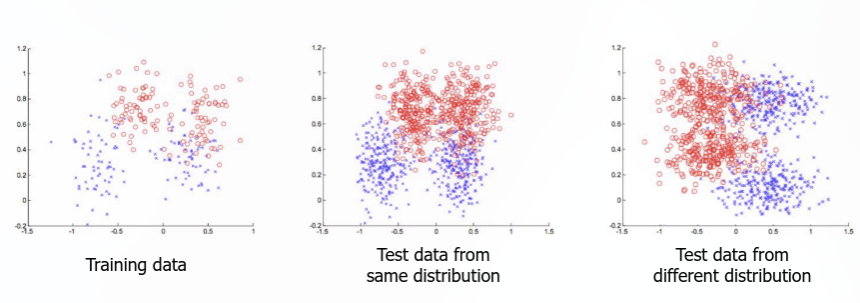
\includegraphics[width=\linewidth]{images/img_20260217_113405.png}
  \caption{Same distribution assumption}
  \label{fig: distrib}
\end{figure}

\newpage

\chapter{Supervised Linear Model}%k
\label{cha:Supervised Linear Model}
\section{Notation}
We denote the $i^{th}$ data sample (input) in the collection of $N$ samples as 
\[ x_i \in \mathbb{R}^D ,\]
a column vector of dimension D.\\ 
We denote the $i^{th}$ label (output) in the collection of $N$ samples as $y_i$.\\
$y_i$ :
\begin{itemize}
  \item for classification represents the category the sample belongs to.
  \item for regression, it can be a single continuous value, or a column vector of dim C.
\end{itemize}

Example:\\
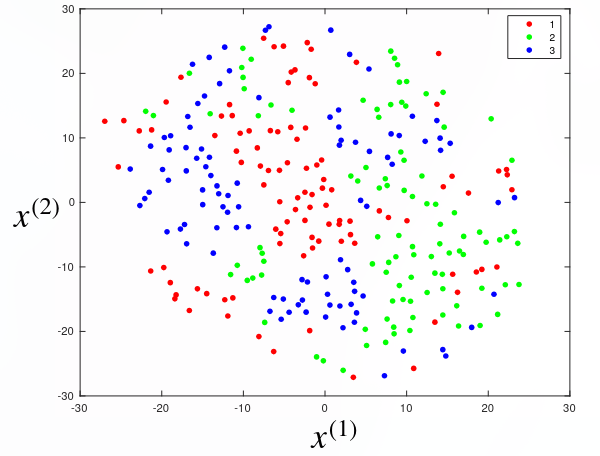
\includegraphics[width=0.5\linewidth]{images/img_20260217_114947.png}\\ 
Here, $x_i$ is one 2D point and thus D = 2, $y_i$ is a discrete value indicating the class (color), i.e, 1, 2 or 3.

\section{Linear Regression}
\subsection{Training}%
\label{sub:Training}
Given $N$ annotated data samples {($x_i,y_i$)} with measurements, we can plot the data, and we will approximate it with a line. Our goal is to find the line that bests fits these measurements \textrightarrow linear regression.
It consists of finding the best line parameters $w^{\left(0\right)*}$ and $w^{\left(1\right)*}$ for some given data.\\ 
This corresponds to the training stage: \\
Given $N$ training pairs { $\left(x_i, y_i\right)$ } , we aim to find $\left(w^{\left(0\right)}, w^{\left(1\right)}\right)$, s.t the predictions of the model 
\[\hat{y_i} = w^{\left(0\right)} + w^{\left(1\right)}x_i\] are close to the true values $y_i$.

The mesure of closeness/error between $y_i$ and $\hat{y_i}$ is represented by the Euclidean distance: \\ 
\[d\left(\hat{y_i},y_i\right) = \sqrt{\left(\hat{y_i} - y_i\right)^2}\]

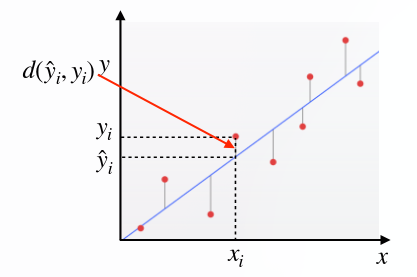
\includegraphics[width=0.6\linewidth]{images/img_20260217_173521.png}

$\hat{y_i} - y_i$ : often reffered to as the \textit{residual}\\ 

In practice, one often prefers using the squared Euclidian distance 
\[d^2\left(\hat{y_i}, y_i\right) = \left(\hat{y_i} - y_i\right)^2\]

Training can then be expressed as the least-squared minization problem 
\[ min_{w^{\left(0\right)}, w^{\left(1\right)}} \frac{1}{N} \sum_{i= 1}^{N} d^2{\left(\hat{y_i},y_i\right)} \]

\subsection{Prediction}%
\label{sub:Prediction}
Once the best line for the given \textit{N} observations is found, we can use it to predict a y value for a new x.\\
Let $w^{\left(0\right)*}$ and $w^{\left(1\right)*}$ be the best line parameters given the observations. \\ 
Then 
\[\hat{y} = w^{\left(0\right)*} + w^{\left(1\right)*}x\] is the estimate value of y for any x.

